% ---------------------------------------------------------
% Vorlage abschlussarbeit.tex
%
% Erstellen: pdflatex, biber, pdflatex, pdflatex
%
% Formatierung für doppelseitigen Druck (dringend empfohlen)
%
% Nutzungshinweis zum Hochschullogo:
%
% Das Logo kann, muss aber nicht auf der Titelseite der Abschlussarbeit
% stehen. Größe und Position des Logos sollen nicht verändert werden; die
% Überlappung mit dem Text ist beabsichtigt. Die Erlaubnis zur Nutzung des
% Logos erstreckt sich nur auf die Abschlussarbeit.
%
% Volker Ahlers, Hochschule Hannover, 2013-2020
% ---------------------------------------------------------

\documentclass[11pt,DIV12,BCOR0mm,twoside,openright,headings=normal,%
  numbers=noenddot,headsepline,headinclude]{scrreprt}
\usepackage[automark,headsepline]{scrpage2}
\usepackage{scrhack}                % to avoid KOMA-Script warning
\usepackage[utf8]{inputenc}         % UTF8 encoding
\usepackage[T1]{fontenc}
\usepackage{txfonts}                % Postscript fonts
\usepackage[ngerman,english]{babel}
\usepackage[style=numeric-comp,giveninits=true,maxnames=10,sorting=none]{biblatex}
\usepackage{graphicx}
\usepackage[usenames]{xcolor}
\usepackage{listings}
\usepackage[pdftex]{hyperref}       % provides \url
\usepackage{wallpaper}              % for HsH logo

% ---------------------------------------------------------

% include only selected chapters
%\includeonly{kapitel_1}

% ---------------------------------------------------------

% package configuration
% biblatex
\addbibresource{literatur.bib}
% scrpage2
\KOMAoptions{headinclude}       
% listings
\lstset{numbers=left,showstringspaces=false,language=Java,%
  basicstyle=\ttfamily,frame=single,rulecolor=\color{gray}}
% hyperref
\hypersetup{linkcolor=black,pdfborder=0 0 0}
\urlstyle{same}

% layout
\tolerance=2000                 % avoid overfull hboxes
\emergencystretch 20pt   
\frenchspacing                  % no extra space after full stops

% HsH logo (optional; do not modify position or size of logo)
\newlength{\HsHOffset}
\setlength{\HsHOffset}{0.05\paperheight}
\newcommand{\HsHLogo}{%
  \AddToShipoutPicture*{%
    \AtPageLowerLeft{%
      \parbox[b]{\paperwidth - \HsHOffset}{%       
        \hfill
        
\includegraphics[height=0.33\paperheight]{hsh-logo}%
        \vspace*{\HsHOffset}%
      }
    }
  }
}

% ---------------------------------------------------------

\begin{document}

\selectlanguage{ngerman}

% title page
\thispagestyle{empty}
\pagenumbering{roman}

\HsHLogo      % optional; do not modify position or size of logo

\begin{center}
  \vspace*{4\baselineskip}
  {\sffamily\bfseries\LARGE
    Titel der Abschlussarbeit
    Titel der Abschlussarbeit
    Titel der Abschlussarbeit\par}
  
  \vspace*{4\baselineskip}
  {\Large Moritz Zeumer}

  \vfill
  {\Large Master-Arbeit}
  
  \vspace*{4\baselineskip}
  {\Large Hochschule Hannover\\
    Fakultät IV -- Wirtschaft und Informatik\\
    Studiengang M.\,Sc.\ Angewandte Informatik\par}
  
  \vspace*{4\baselineskip}
  {\Large 13.\,7.\,2020}
  
  \vspace*{4\baselineskip}
\end{center}

\cleardoublepage

\noindent
{\sffamily\bfseries Autor}					% oder Autorin

\vspace*{.5\baselineskip}
\noindent
Moritz Zeumer\\
Matrikelnummer: 1498947\\
E-Mail: m\_zeumer@gmx.de

\vspace*{1\baselineskip}
\noindent
{\sffamily\bfseries Erstprüfer}				% oder Erstprüferin

\vspace*{.5\baselineskip}
\noindent
Prof. Dr. Volker Ahlers\\
Hochschule Hannover\\
Fakultät IV, Abteilung Informatik\\
Ricklinger Stadtweg 120\\
30459 Hannover

\vspace*{1\baselineskip}
\noindent
{\sffamily\bfseries Zweitprüferin}			% oder Zweitprüfer

\vspace*{.5\baselineskip}
\noindent
Herr Simon Schneegans\\
Deutsches Zentrum für Luft- und Raumfahrt\\
Lilienthalplatz 7\\
38108 Braunschweig

% ggf. Firmenbetreuer_in, falls nicht Zweitprüfer_in

\vfill
\noindent
{\sffamily\bfseries Selbständigkeitserklärung}

\vspace*{.5\baselineskip}
\noindent
Hiermit erkläre ich, dass ich die eingereichte Master-Arbeit selbständig und ohne fremde Hilfe verfasst, andere als die von mir angegebenen Quellen und Hilfsmittel nicht benutzt und die den benutzten Werken wörtlich oder inhaltlich entnommenen Stellen als solche kenntlich gemacht habe.

\vspace*{3\baselineskip}
\noindent
Ort, Datum\hspace{5cm} Unterschrift
% table of contents
\tableofcontents

% main text
\cleardoublepage
\pagenumbering{arabic}

\chapter{Hinweise}

\section{Text und Verweise}

Die folgenden Hinweise sollen Ihnen helfen, eine wissenschaftliche Arbeit zu erstellen.
Das Layout (z.\,B.\ den Rahmen um das Code-Beispiel) dürfen Sie natürlich gemäß Ihren
Vorlieben anpassen.
Mathematische Ausdrücke können im Fließtext als $x^2 = 5$ oder in eigenen Zeilen als
\[
  \int_{-\infty}^\infty f(x)\,dx = \sin(\alpha)
\]
gesetzt werden.
Code-Beispiele sind möglich, sollten aber auf wenige Zeilen beschränkt bleiben.
Im Folgenden wird eine Schleife mit den Variablen \lstinline+sum+ und \lstinline+i+
verwendet.

{\small
\begin{lstlisting}
int sum = 0;
for (int i = 0; i < 10; ++i) {
  sum += i;
}
\end{lstlisting}%
}

\begin{figure}[!htb]
  \centerline{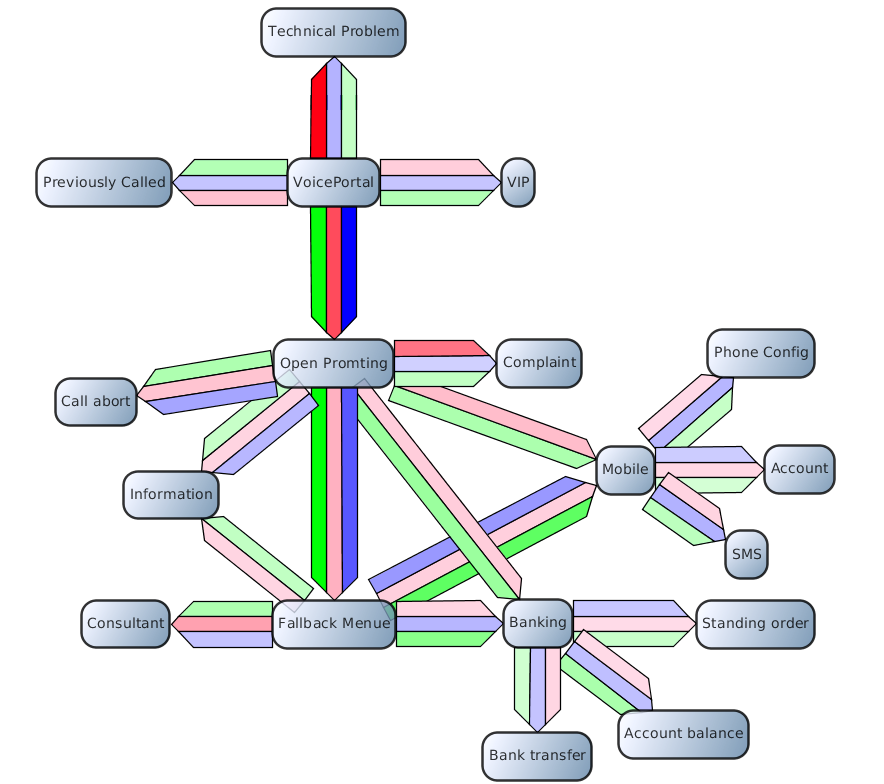
\includegraphics[width=0.5\textwidth]{abbildung_1}}
  \caption{Vergleichende Visualisierung der Nutzerströme zwischen
    Sprachdialogen \cite{Zimmer2011}.}
  \label{abbildung1}
\end{figure}

Auf alle Abbildungen~-- z.\,B.\ Abb.~\ref{abbildung1}~-- wird im Text verwiesen.
Referenzen werden nach der zu belegenden Aussage in eckigen Klammern angegeben
\cite{Bostock2011,D3js,Laemmel2012}.
Für fremde Abbildungen steht die Referenz in der Abbildungsbeschriftung,
siehe Abb.~\ref{abbildung1}.

\section{Vorgehensweise}

Einige Tipps zum Schreiben der Abschlussarbeit:
\begin{itemize}
  \item Stellen Sie eine grobe Zeitplanung auf, ähnlich einem Projektplan mit Meilensteinen,
    und diskutieren Sie diese mit mir.
    Gleiches gilt für die Gliederung der Arbeit.
  \item Bedenken Sie, dass in der Abschlussarbeit Ihre eigene Arbeit im Mittelpunkt stehen
    sollte.
    Einleitende Kapitel und Beschreibungen verwendeter Techniken sollten entsprechend
    knapp ausfallen.
  \item Dass alle verwendeten Literaturquellen angegeben werden müssen, ist Ihnen
    sicher bekannt. Ein Plagiat stellt einen Täuschungsversuch dar, der schwerwiegende Folgen 
    nach sich ziehen kann.
    Wörtliche Zitate sind in Informatikarbeiten unüblich und selten sinnvoll.
    Bei aus Büchern, Artikeln oder von Webseiten übernommenen Abbildungen muss
    die jeweilige Quelle deutlich angegeben werden (s.\,o.).
  \item Nutzen Sie zur Literaturrecherche die aus dem HsH-Netz zugänglichen Datenbanken
    ACM Digital Library\footnote{\url{https://dl.acm.org/}} und IEEE Xplore\footnote{\url{https://ieeexplore.ieee.org/}}.
    Wikipedia ist praktisch zur Begriffsklärung oder für einen ersten Einstieg in ein Thema,
    stellt aber keine wissenschaftliche Quelle dar; zitieren Sie stattdessen Lehrbücher
    oder Artikel aus Fachzeitschriften oder Konferenzbänden.
  \item Geben Sie vollständige Literaturangaben an:
    \begin{itemize}
      \item Autor, Titel, Erscheinungsjahr
      \item Buch mit Verlag, Verlagsort und Auflage (engl. \emph{edition}, nur anzugeben,
       falls $>1$)
      \item Zeitschrift/Konferenzband mit Bandnummer (engl. \emph{volume}, sofern vorhanden)
         und Seitenzahlen
      \item Abschlussarbeiten etc. mit Hochschule und Art des Textes (Doktorarbeit,
        Master-Arbeit, Seminararbeit o.\,ä.)
      \item Internetquellen mit URL und Datum des Abrufs
    \end{itemize}
    Beispiele finden Sie im Literaturverzeichnis dieses Textes oder in Lehrbüchern.
  \item Den einen richtigen Zitierstil gibt es nicht.
    Definitiv unüblich ist in der Informatik aber die in den Geisteswissenschaften bevorzugte
    Variante mit Fußnoten; lassen Sie sich von möglichen KorrekturleserInnen aus anderen
    Fachrichtungen nichts einreden.
  \item Sie können mir gern zwischendurch Vorabversionen Ihrer Arbeit zur Durchsicht
    einreichen.
    Dies empfiehlt sich bereits, wenn Sie die ersten Abschnitte ausformuliert
    haben, damit ich frühzeitig auf mögliche Fehler hinweisen kann; sehr grobe Entwürfe
    (Stichwortsammlungen) nehme ich allerdings nicht an.
    Ich gebe Ihnen Hinweise zur Verbesserung, führe jedoch keine Rechtschreib- und
    Grammatikkorrektur durch.
    
    \emph{Wichtig:} Bitte wählen Sie einen Dateinamen, aus dem Ihr Name und das Datum der
    aktuellen Version hervorgehen (z.\,B.\ \verb+bachelor-arbeit_meyer_20160613.pdf+).
  \item Am Ende wird natürlich Ihre eigene Arbeit bewertet.
    Auch wenn Sie alle meine Vorschläge berücksichtigen, führt dies nicht zwangsläufig zu
    einer Benotung mit 1,0.
\end{itemize}

Weitere Hinweise finden Sie im Moodle-Kurs "`Abschlussarbeiten der Abteilung
Informatik"'.\footnote{\url{https://moodle.hs-hannover.de/course/view.php?id=6530}}

\vspace{\baselineskip}
\emph{Wird fortgesetzt \ldots}



\chapter{Text}

Text Text Text Text Text Text Text Text Text Text Text Text Text Text Text 
Text Text Text Text Text Text Text Text Text Text Text Text Text Text Text 
Text Text Text Text Text Text Text Text Text Text Text Text Text Text Text 
Text Text Text Text Text Text Text Text Text Text Text Text Text Text Text 
Text Text Text Text Text Text Text Text Text Text Text Text Text Text Text 
Text Text Text Text Text Text Text Text Text Text Text Text Text Text Text 
Text Text Text Text Text Text Text Text Text Text Text Text Text Text Text 
Text Text Text Text Text Text Text Text Text Text Text Text Text Text Text 
Text Text Text Text Text Text Text Text Text Text Text Text Text Text Text 

\section{Text}

Text Text Text Text Text Text Text Text Text Text Text Text Text Text Text 
Text Text Text Text Text Text Text Text Text Text Text Text Text Text Text 
Text Text Text Text Text Text Text Text Text Text Text Text Text Text Text 
Text Text Text Text Text Text Text Text Text Text Text Text Text Text Text 
Text Text Text Text Text Text Text Text Text Text Text Text Text Text Text 
Text Text Text Text Text Text Text Text Text Text Text Text Text Text Text 
Text Text Text Text Text Text Text Text Text Text Text Text Text Text Text 
Text Text Text Text Text Text Text Text Text Text Text Text Text Text Text 
Text Text Text Text Text Text Text Text Text Text Text Text Text Text Text 

Text Text Text Text Text Text Text Text Text Text Text Text Text Text Text 
Text Text Text Text Text Text Text Text Text Text Text Text Text Text Text 
Text Text Text Text Text Text Text Text Text Text Text Text Text Text Text 
Text Text Text Text Text Text Text Text Text Text Text Text Text Text Text 
Text Text Text Text Text Text Text Text Text Text Text Text Text Text Text 
Text Text Text Text Text Text Text Text Text Text Text Text Text Text Text 
Text Text Text Text Text Text Text Text Text Text Text Text Text Text Text 
Text Text Text Text Text Text Text Text Text Text Text Text Text Text Text 
Text Text Text Text Text Text Text Text Text Text Text Text Text Text Text 

Text Text Text Text Text Text Text Text Text Text Text Text Text Text Text 
Text Text Text Text Text Text Text Text Text Text Text Text Text Text Text 
Text Text Text Text Text Text Text Text Text Text Text Text Text Text Text 
Text Text Text Text Text Text Text Text Text Text Text Text Text Text Text 
Text Text Text Text Text Text Text Text Text Text Text Text Text Text Text 
Text Text Text Text Text Text Text Text Text Text Text Text Text Text Text 
Text Text Text Text Text Text Text Text Text Text Text Text Text Text Text 
Text Text Text Text Text Text Text Text Text Text Text Text Text Text Text 
Text Text Text Text Text Text Text Text Text Text Text Text Text Text Text 

Text Text Text Text Text Text Text Text Text Text Text Text Text Text Text 
Text Text Text Text Text Text Text Text Text Text Text Text Text Text Text 
Text Text Text Text Text Text Text Text Text Text Text Text Text Text Text 
Text Text Text Text Text Text Text Text Text Text Text Text Text Text Text 
Text Text Text Text Text Text Text Text Text Text Text Text Text Text Text 
Text Text Text Text Text Text Text Text Text Text Text Text Text Text Text 
Text Text Text Text Text Text Text Text Text Text Text Text Text Text Text 
Text Text Text Text Text Text Text Text Text Text Text Text Text Text Text 
Text Text Text Text Text Text Text Text Text Text Text Text Text Text Text 

\section{Mehr Text}

Text Text Text Text Text Text Text Text Text Text Text Text Text Text Text 
Text Text Text Text Text Text Text Text Text Text Text Text Text Text Text 
Text Text Text Text Text Text Text Text Text Text Text Text Text Text Text 
Text Text Text Text Text Text Text Text Text Text Text Text Text Text Text 
Text Text Text Text Text Text Text Text Text Text Text Text Text Text Text 
Text Text Text Text Text Text Text Text Text Text Text Text Text Text Text 
Text Text Text Text Text Text Text Text Text Text Text Text Text Text Text 
Text Text Text Text Text Text Text Text Text Text Text Text Text Text Text 
Text Text Text Text Text Text Text Text Text Text Text Text Text Text Text 

Text Text Text Text Text Text Text Text Text Text Text Text Text Text Text 
Text Text Text Text Text Text Text Text Text Text Text Text Text Text Text 
Text Text Text Text Text Text Text Text Text Text Text Text Text Text Text 
Text Text Text Text Text Text Text Text Text Text Text Text Text Text Text 
Text Text Text Text Text Text Text Text Text Text Text Text Text Text Text 
Text Text Text Text Text Text Text Text Text Text Text Text Text Text Text 
Text Text Text Text Text Text Text Text Text Text Text Text Text Text Text 
Text Text Text Text Text Text Text Text Text Text Text Text Text Text Text 
Text Text Text Text Text Text Text Text Text Text Text Text Text Text Text 

Text Text Text Text Text Text Text Text Text Text Text Text Text Text Text 
Text Text Text Text Text Text Text Text Text Text Text Text Text Text Text 
Text Text Text Text Text Text Text Text Text Text Text Text Text Text Text 
Text Text Text Text Text Text Text Text Text Text Text Text Text Text Text 
Text Text Text Text Text Text Text Text Text Text Text Text Text Text Text 
Text Text Text Text Text Text Text Text Text Text Text Text Text Text Text 
Text Text Text Text Text Text Text Text Text Text Text Text Text Text Text 
Text Text Text Text Text Text Text Text Text Text Text Text Text Text Text 
Text Text Text Text Text Text Text Text Text Text Text Text Text Text Text 

Text Text Text Text Text Text Text Text Text Text Text Text Text Text Text 
Text Text Text Text Text Text Text Text Text Text Text Text Text Text Text 
Text Text Text Text Text Text Text Text Text Text Text Text Text Text Text 
Text Text Text Text Text Text Text Text Text Text Text Text Text Text Text 
Text Text Text Text Text Text Text Text Text Text Text Text Text Text Text 
Text Text Text Text Text Text Text Text Text Text Text Text Text Text Text 
Text Text Text Text Text Text Text Text Text Text Text Text Text Text Text 
Text Text Text Text Text Text Text Text Text Text Text Text Text Text Text 
Text Text Text Text Text Text Text Text Text Text Text Text Text Text Text 


% appendix (optional}
\appendix

\chapter{Text}

Anhänge werden mit Buchstaben nummeriert und sind z.\,B. sinnvoll für
größere Code-Ausschnitte,
Beispiele für Konfigurationsdateien, Bedienungshinweise etc.

\section{Text}

Text Text Text Text Text Text Text Text Text Text Text Text Text Text Text 
Text Text Text Text Text Text Text Text Text Text Text Text Text Text Text 
Text Text Text Text Text Text Text Text Text Text Text Text Text Text Text 
Text Text Text Text Text Text Text Text Text Text Text Text Text Text Text 
Text Text Text Text Text Text Text Text Text Text Text Text Text Text Text 
Text Text Text Text Text Text Text Text Text Text Text Text Text Text Text 
Text Text Text Text Text Text Text Text Text Text Text Text Text Text Text 
Text Text Text Text Text Text Text Text Text Text Text Text Text Text Text 
Text Text Text Text Text Text Text Text Text Text Text Text Text Text Text 

Text Text Text Text Text Text Text Text Text Text Text Text Text Text Text 
Text Text Text Text Text Text Text Text Text Text Text Text Text Text Text 
Text Text Text Text Text Text Text Text Text Text Text Text Text Text Text 
Text Text Text Text Text Text Text Text Text Text Text Text Text Text Text 
Text Text Text Text Text Text Text Text Text Text Text Text Text Text Text 
Text Text Text Text Text Text Text Text Text Text Text Text Text Text Text 
Text Text Text Text Text Text Text Text Text Text Text Text Text Text Text 
Text Text Text Text Text Text Text Text Text Text Text Text Text Text Text 
Text Text Text Text Text Text Text Text Text Text Text Text Text Text Text 

Text Text Text Text Text Text Text Text Text Text Text Text Text Text Text 
Text Text Text Text Text Text Text Text Text Text Text Text Text Text Text 
Text Text Text Text Text Text Text Text Text Text Text Text Text Text Text 
Text Text Text Text Text Text Text Text Text Text Text Text Text Text Text 
Text Text Text Text Text Text Text Text Text Text Text Text Text Text Text 
Text Text Text Text Text Text Text Text Text Text Text Text Text Text Text 
Text Text Text Text Text Text Text Text Text Text Text Text Text Text Text 
Text Text Text Text Text Text Text Text Text Text Text Text Text Text Text 
Text Text Text Text Text Text Text Text Text Text Text Text Text Text Text 

\section{Mehr Text}

Text Text Text Text Text Text Text Text Text Text Text Text Text Text Text 
Text Text Text Text Text Text Text Text Text Text Text Text Text Text Text 
Text Text Text Text Text Text Text Text Text Text Text Text Text Text Text 
Text Text Text Text Text Text Text Text Text Text Text Text Text Text Text 
Text Text Text Text Text Text Text Text Text Text Text Text Text Text Text 
Text Text Text Text Text Text Text Text Text Text Text Text Text Text Text 
Text Text Text Text Text Text Text Text Text Text Text Text Text Text Text 
Text Text Text Text Text Text Text Text Text Text Text Text Text Text Text 
Text Text Text Text Text Text Text Text Text Text Text Text Text Text Text 

Text Text Text Text Text Text Text Text Text Text Text Text Text Text Text 
Text Text Text Text Text Text Text Text Text Text Text Text Text Text Text 
Text Text Text Text Text Text Text Text Text Text Text Text Text Text Text 
Text Text Text Text Text Text Text Text Text Text Text Text Text Text Text 
Text Text Text Text Text Text Text Text Text Text Text Text Text Text Text 
Text Text Text Text Text Text Text Text Text Text Text Text Text Text Text 
Text Text Text Text Text Text Text Text Text Text Text Text Text Text Text 
Text Text Text Text Text Text Text Text Text Text Text Text Text Text Text 
Text Text Text Text Text Text Text Text Text Text Text Text Text Text Text 

Text Text Text Text Text Text Text Text Text Text Text Text Text Text Text 
Text Text Text Text Text Text Text Text Text Text Text Text Text Text Text 
Text Text Text Text Text Text Text Text Text Text Text Text Text Text Text 
Text Text Text Text Text Text Text Text Text Text Text Text Text Text Text 
Text Text Text Text Text Text Text Text Text Text Text Text Text Text Text 
Text Text Text Text Text Text Text Text Text Text Text Text Text Text Text 
Text Text Text Text Text Text Text Text Text Text Text Text Text Text Text 
Text Text Text Text Text Text Text Text Text Text Text Text Text Text Text 
Text Text Text Text Text Text Text Text Text Text Text Text Text Text Text 

Text Text Text Text Text Text Text Text Text Text Text Text Text Text Text 
Text Text Text Text Text Text Text Text Text Text Text Text Text Text Text 
Text Text Text Text Text Text Text Text Text Text Text Text Text Text Text 
Text Text Text Text Text Text Text Text Text Text Text Text Text Text Text 
Text Text Text Text Text Text Text Text Text Text Text Text Text Text Text 
Text Text Text Text Text Text Text Text Text Text Text Text Text Text Text 
Text Text Text Text Text Text Text Text Text Text Text Text Text Text Text 
Text Text Text Text Text Text Text Text Text Text Text Text Text Text Text 
Text Text Text Text Text Text Text Text Text Text Text Text Text Text Text 

Text Text Text Text Text Text Text Text Text Text Text Text Text Text Text 
Text Text Text Text Text Text Text Text Text Text Text Text Text Text Text 
Text Text Text Text Text Text Text Text Text Text Text Text Text Text Text 
Text Text Text Text Text Text Text Text Text Text Text Text Text Text Text 
Text Text Text Text Text Text Text Text Text Text Text Text Text Text Text 
Text Text Text Text Text Text Text Text Text Text Text Text Text Text Text 
Text Text Text Text Text Text Text Text Text Text Text Text Text Text Text 
Text Text Text Text Text Text Text Text Text Text Text Text Text Text Text 
Text Text Text Text Text Text Text Text Text Text Text Text Text Text Text 


% bibliography
% Wichtig: Das Literaturverzeichnis steht ganz am Ende der Arbeit, also nach
% einem möglichen Anhang.
\addcontentsline{toc}{chapter}{Literaturverzeichnis}
\printbibliography

\end{document}
